\chapter{Additional Experiments}
\label{app:ch:additional_experiments}
% \section{WIP --- EDM-CSDI Sampling exploration}
In this chapter, we discuss some of the explorations conducted to assess whether sample improvements are possible and how the model behaves when stochasticity is re-introduced during the generation phase.

 Three sampling explorations were covered: the second-order Heun stochastic sampler (Heun SDE for brevity), the \(\sigma_{\max}\) sampler prior, and an NFEs exploration. Specifically, the first evaluates whether the model can recover some peculiarities of FTS paths through the injection of stochasticity; the second explores whether a prior further from or closer to the original distribution may influence sampling quality while retaining the same computational cost; and the last checks whether the reconstruction error is already under control with the current settings (\(NFEs=400\) or \(steps=200\)), or whether there is margin for improvement or reduction, given that this was an upper bound.
\subsection{Heun Stochastic Sampler}
In the first phase, we generated data under the same conditions as sub-Sec.\ \ref{subsec:conditiona_edm_csdi}, using EDM-CSDI (Cond.) with a stochastic sampler instead. Specifically, we experimented with a budget of \(S_{\text{churn}}=10\), \(S_{\text{tmin}}=0.05\), \(S_{\text{tmax}}=\infty\), and \(S_{\text{noise}}=1.0\). Over \(20,000\) windows, the distributional properties remained largely unchanged.

\begin{table}[htbp]
\centering
\footnotesize
\renewcommand{\arraystretch}{1.3}
\setlength{\tabcolsep}{4.5pt}
\begin{tabular}{
  % l
  l
  S[table-format= 1.4]   % Mean:     ±0.xxxx
  S[table-format= 1.5]   % Std:      0.xxxxx
  S[table-format=-1.4]   % Skew.:   -x.xxxx
  S[table-format= 2.1]   % Kur.: xx.x
  S[table-format=-1.4]   % q01:     -x.xxxx
  S[table-format= 1.4]   % q99:      x.xxxx
}
\toprule
    \textbf{Sampler}
  & {\textbf{Mean}}
  & {\textbf{Std}}
  & {\textbf{Skew.}}
  & {\textbf{Kur.}}
  & {$\boldsymbol{q_{0.01}}$}
  & {$\boldsymbol{q_{0.99}}$} \\
\midrule
Reference    &  0.0000 & 1.0000 & -0.5864 & 39.5 & -2.7188 & 2.7784 \\
Heun ODE     &  0.0029 & 0.9487 & -0.5390 & 39.0 & -2.5789 & 2.6306 \\
Heun SDE     &  0.0012 & 1.0041 & -0.6876 & 45.6 & -2.7224 & 2.7662 \\
\bottomrule
\end{tabular}
\caption{Aggregate statistics for EDM-CSDI (Cond.) under the deterministic Heun ODE and stochastic Heun (SDE, $S_{\mathrm{churn}}=10$) samplers, normalized log-returns. This is for combined windows.}
\label{tab:sampler_experiment}
\end{table}

\begin{table}[htbp]
\centering
\footnotesize
\renewcommand{\arraystretch}{1.3}
\setlength{\tabcolsep}{4.5pt}
\begin{tabular}{
  % l
  l
  % S[table-format= 1.4]   % Mean:     ±0.xxxx
  % S[table-format= 1.5]   % Std:      0.xxxxx
  % S[table-format=-1.4]   % Skew.:   -x.xxxx
  % S[table-format= 2.4]   % Ex.Kurt.: xx.xxxx
  % S[table-format=-1.4]   % q01:     -x.xxxx
  % S[table-format= 1.4]   % q99:      x.xxxx
  l
  l
  % S[table-format= 2]   % KS:       x.xxx
  % S[table-format= 2]   % W1:       x.xxx
  l                      % alpha:    blank
}
\toprule
    \textbf{Sampler}
  & {$D_{\mathrm{KS}}$}
  & {$W_1$}
  & {$\hat{\alpha}$} \\
\midrule
Reference & {---} & {---} & 4.418 \\
Heun ODE &  0.0411 & 0.000569 & 4.572 \\
Heun SDE &  0.0377 & 0.000077 & \\
\bottomrule
\end{tabular}
\caption{Distributional similarity metrics ($D_{\mathrm{KS}}$, $W_1$, $\hat{\alpha}$) for EDM-CSDI (Cond.) under the Heun ODE/SDE samplers (cf.\ Tab.~\ref{tab:sampler_experiment}).}
\label{tab:edm_sampler_distributional_metrics}
\end{table}

As shown in Tab.\ \ref{tab:sampler_experiment} and Tab.\ \ref{tab:edm_sampler_distributional_metrics}, the advantage of using SDE is that the injection of noise brings new possible trajectories, increasing the standard deviation. While this is positive, as it brings us closer to the original distribution, it also causes kurtosis to increase and skewness to grow beyond the reference. This is probably due to the stochasticity pushing the model into regions that are seldomly seen, hence poorly learned.

\textbf{Stylized Facts} \quad Fig.\ \ref{fig:sampler_stylized_facts} compares the heavy-tail distribution, volatility clustering, and leverage effect obtained with the Heun ODE and Heun SDE samplers against the Reference. The Heun SDE sampler generated paths display somewhat more variability in leverage effects, while matching Heun ODE and Reference properties.

\begin{figure}[htbp]
    \centering
    \begin{subfigure}{0.32\textwidth}
        \centering
        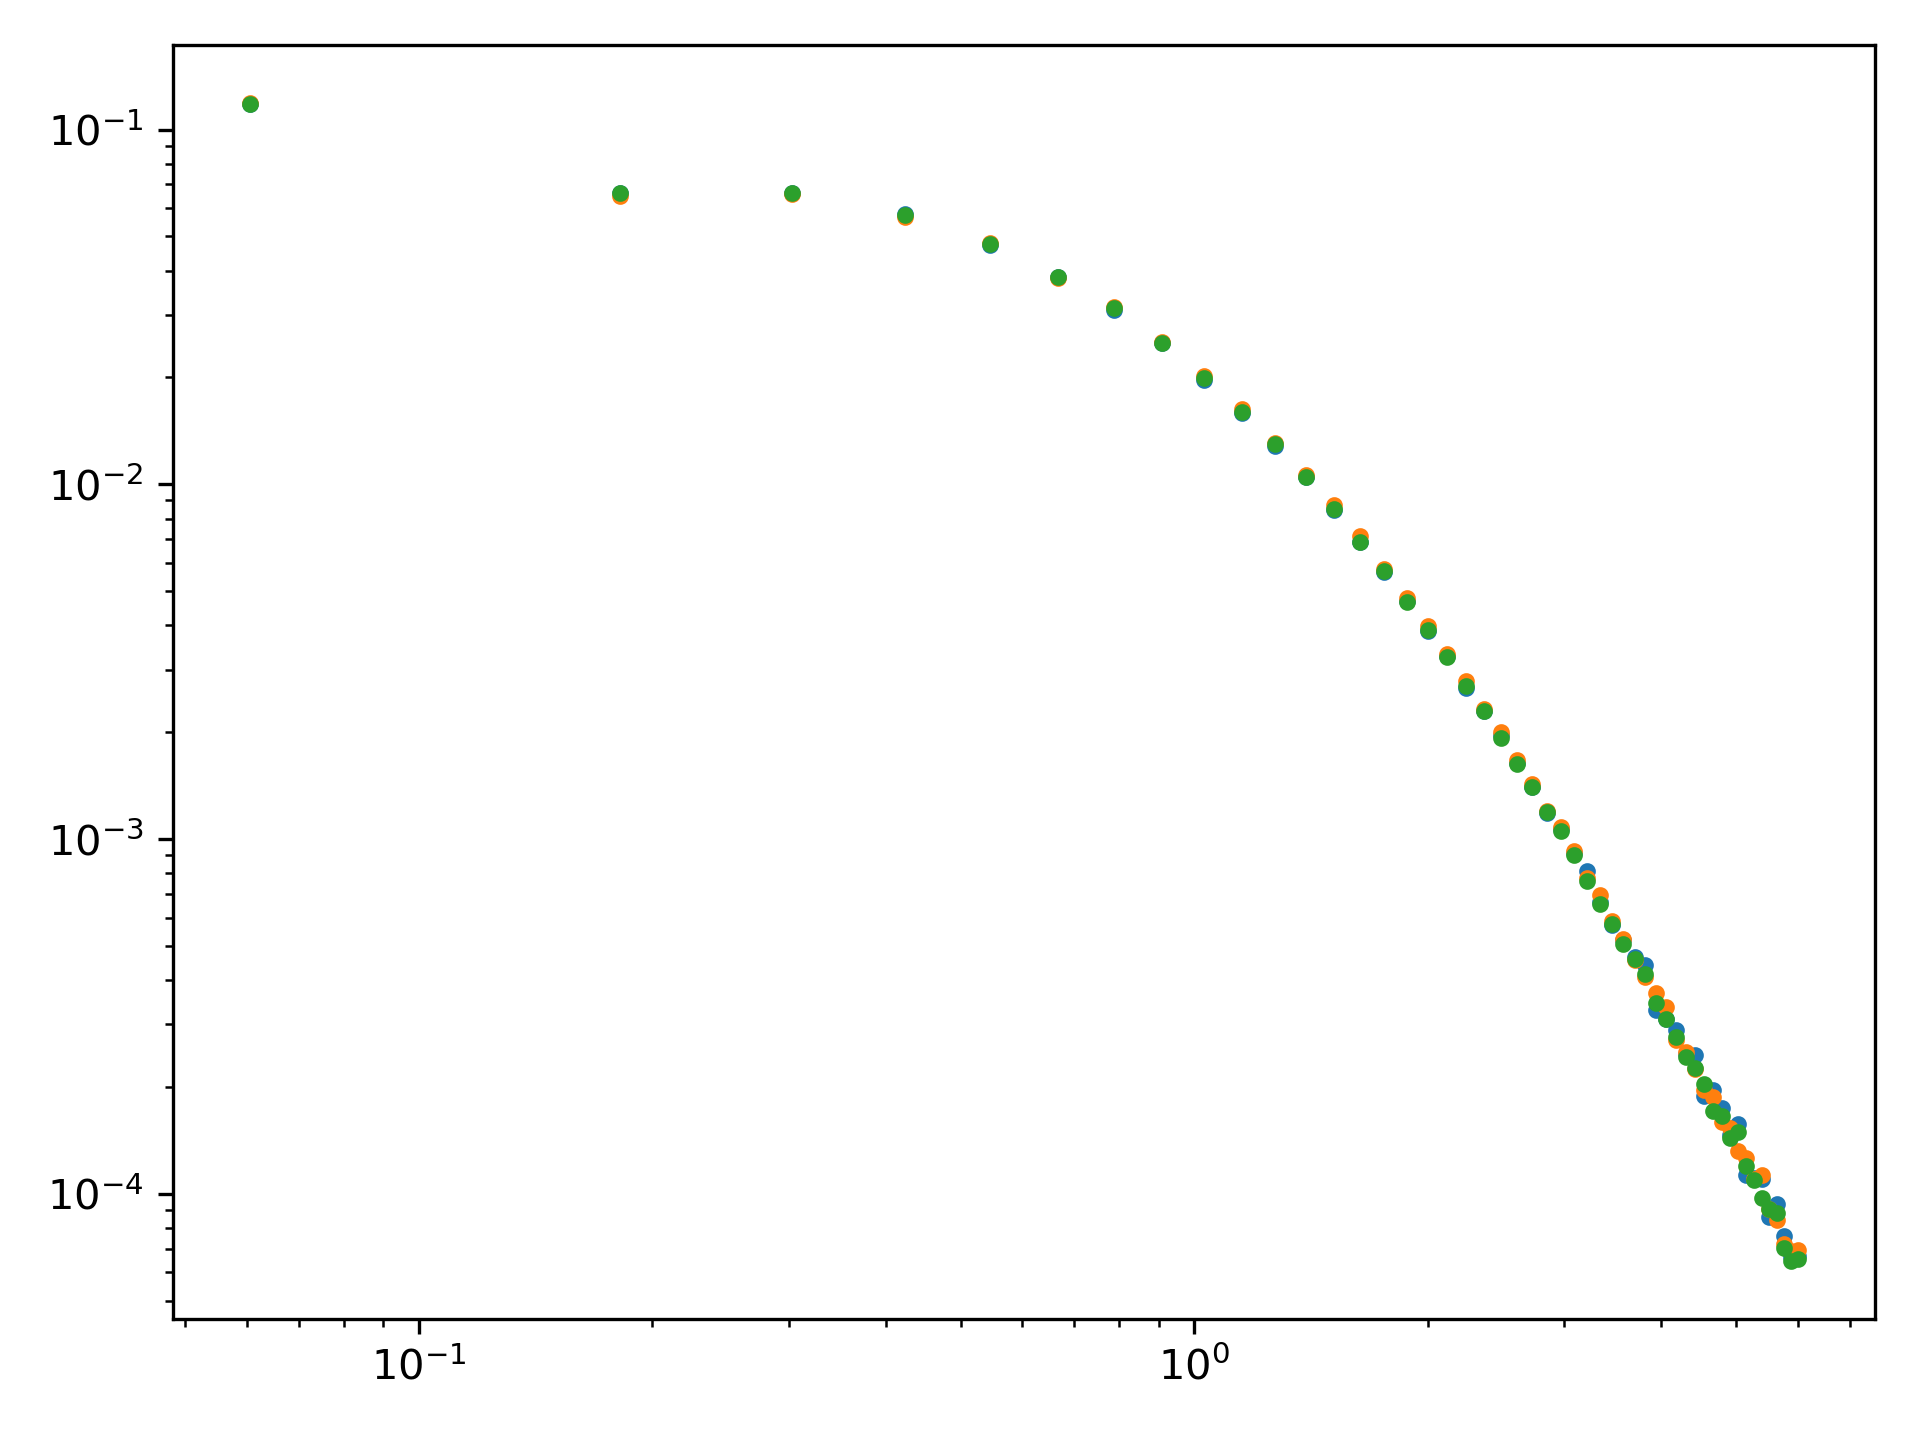
\includegraphics[width=\linewidth]{images/extra_experiments/overlap_distribution_pos_ref_ODE_SDE.png}
        \label{fig:sampler_tail}
    \end{subfigure}
    \hfill
    \begin{subfigure}{0.32\textwidth}
        \centering
        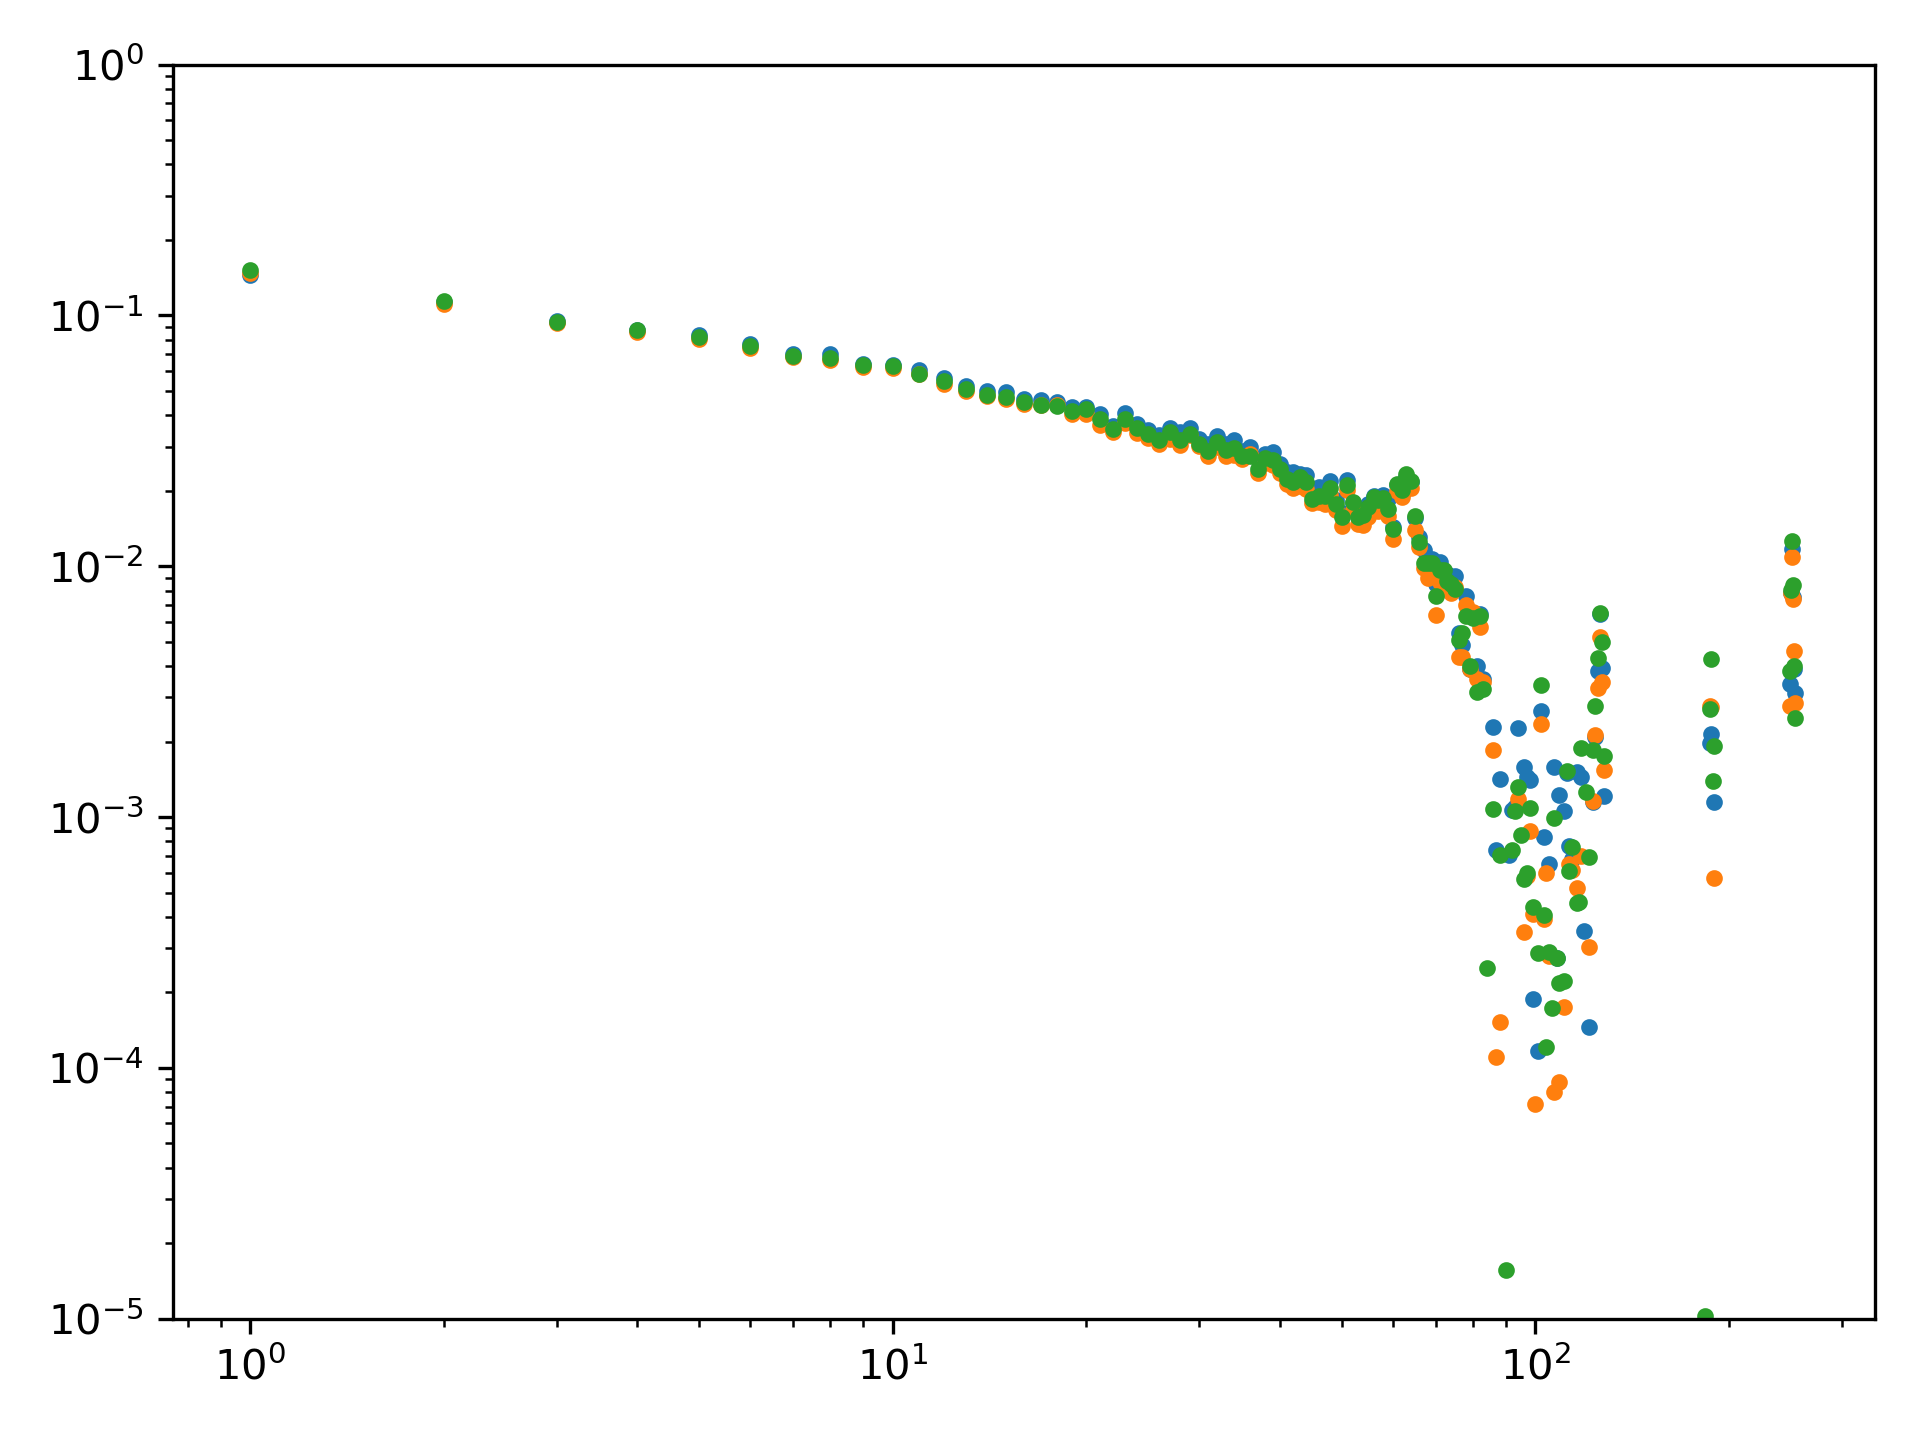
\includegraphics[width=\linewidth]{images/extra_experiments/overlap_acf_ref_ODE_SDE.png}
        \label{fig:sampler_vol}
    \end{subfigure}
    \hfill
    \begin{subfigure}{0.32\textwidth}
        \centering
        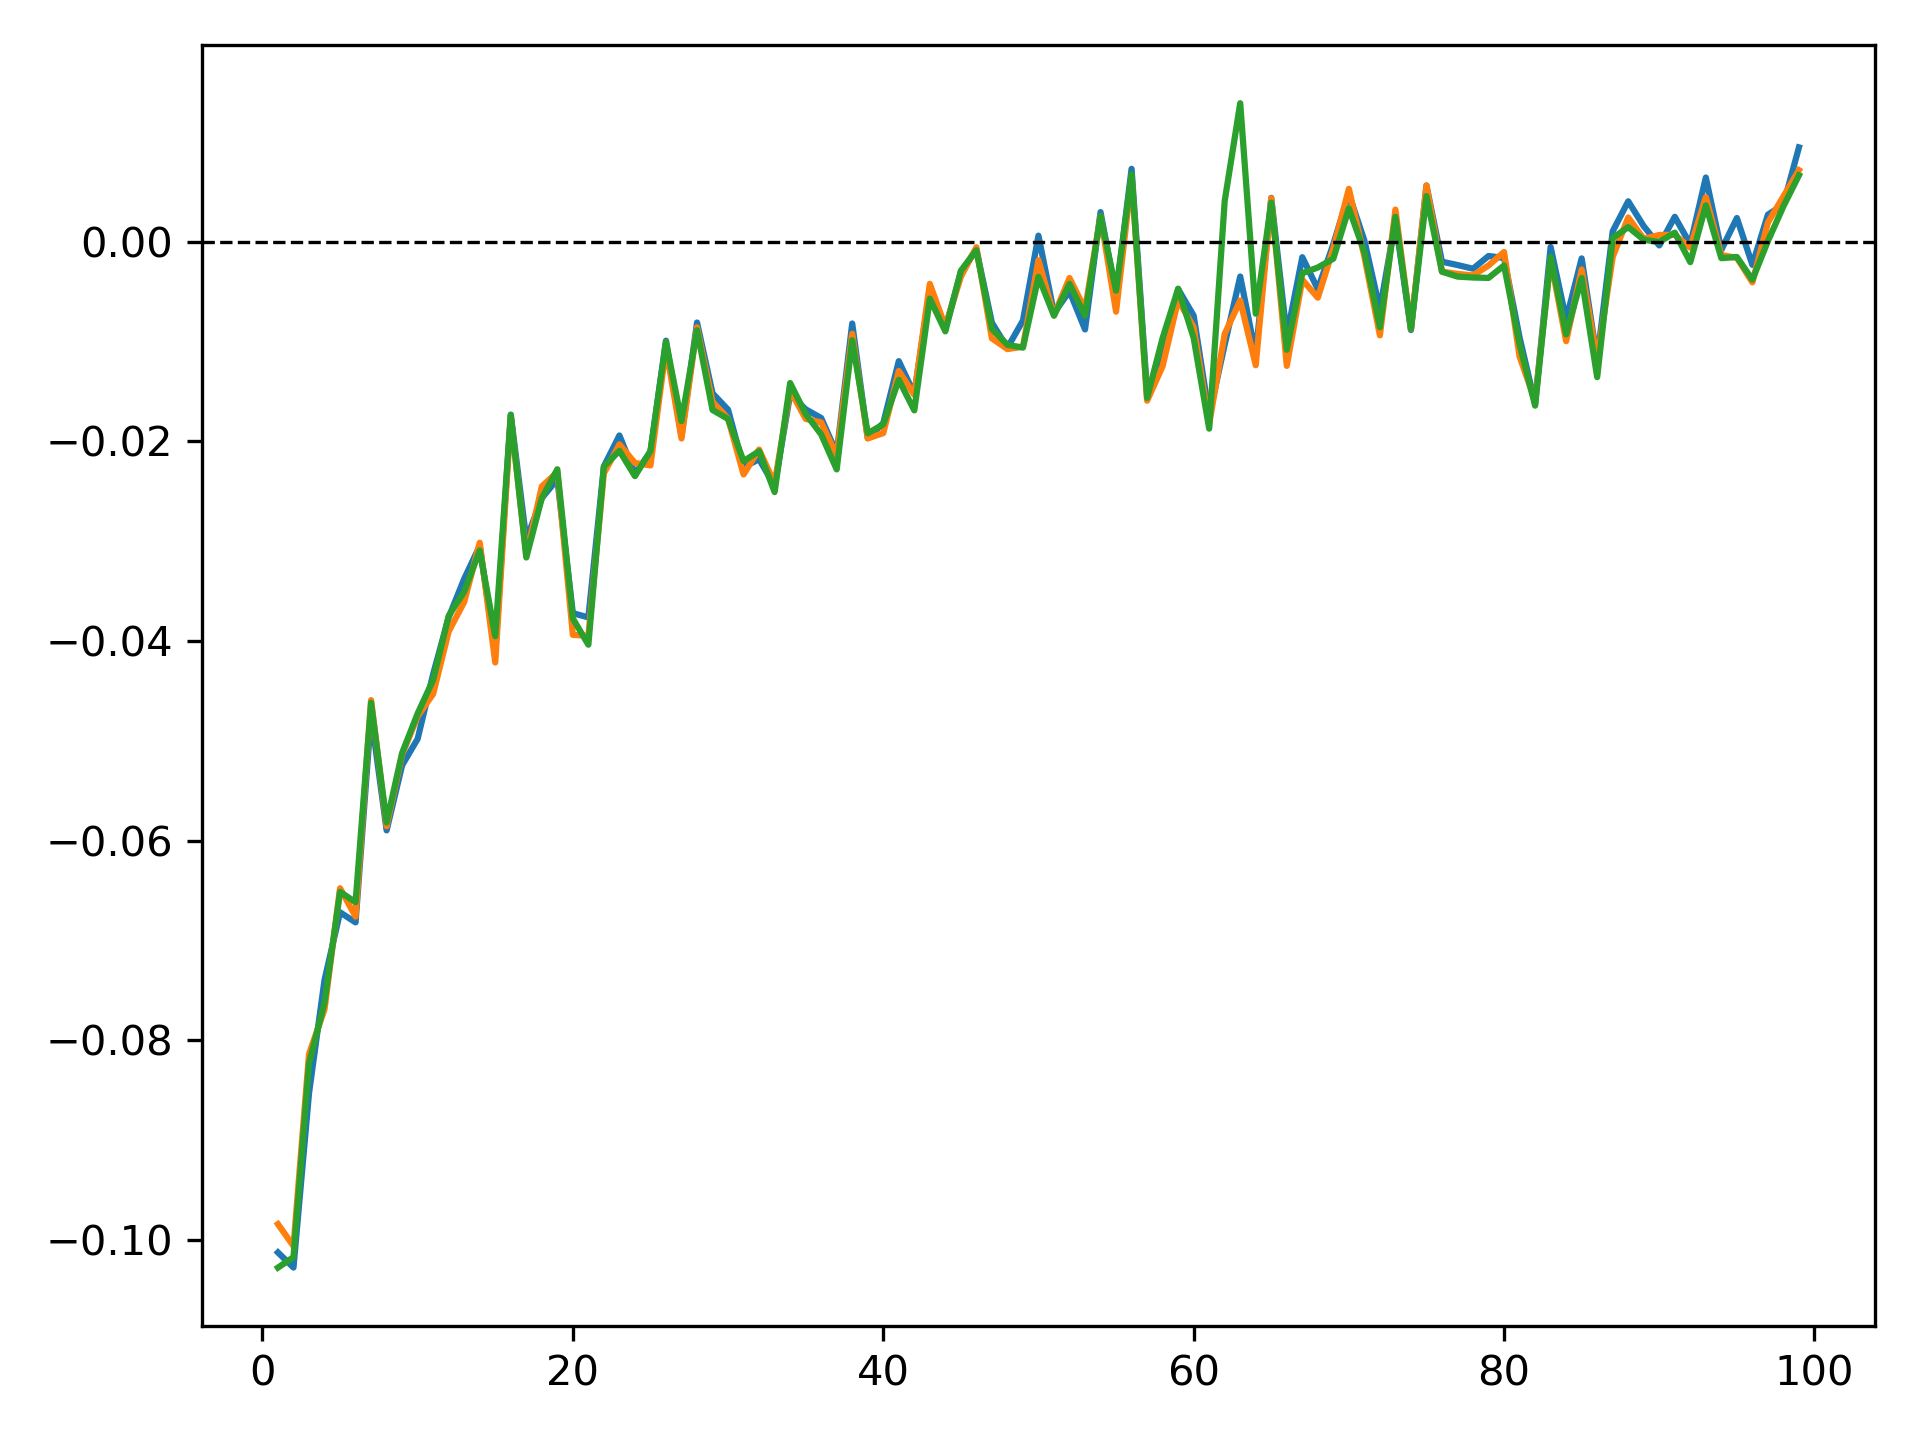
\includegraphics[width=\linewidth]{images/extra_experiments/overlap_leverage_ref_ODE_SDE.png}
        \label{fig:sampler_leverage}
    \end{subfigure}

    \caption{Stylized facts for EDM-CSDI (Cond.) under the Heun ODE (orange) and Heun SDE (green) samplers, against the Reference (blue). From left to right: heavy-tail distribution, volatility clustering, leverage effect.}
    \label{fig:sampler_stylized_facts}
\end{figure}

\textbf{Price Paths Samples} \quad Fig.\ \ref{fig:sampler_price_paths} illustrates sample price paths generated under the Heun ODE and Heun SDE samplers against the Ground Truth were it is possible to observe that SDE carries more variability and breadth in its generated paths.

\begin{figure}[htbp]
    \centering
    \begin{subfigure}[c]{0.32\textwidth}
        \centering
        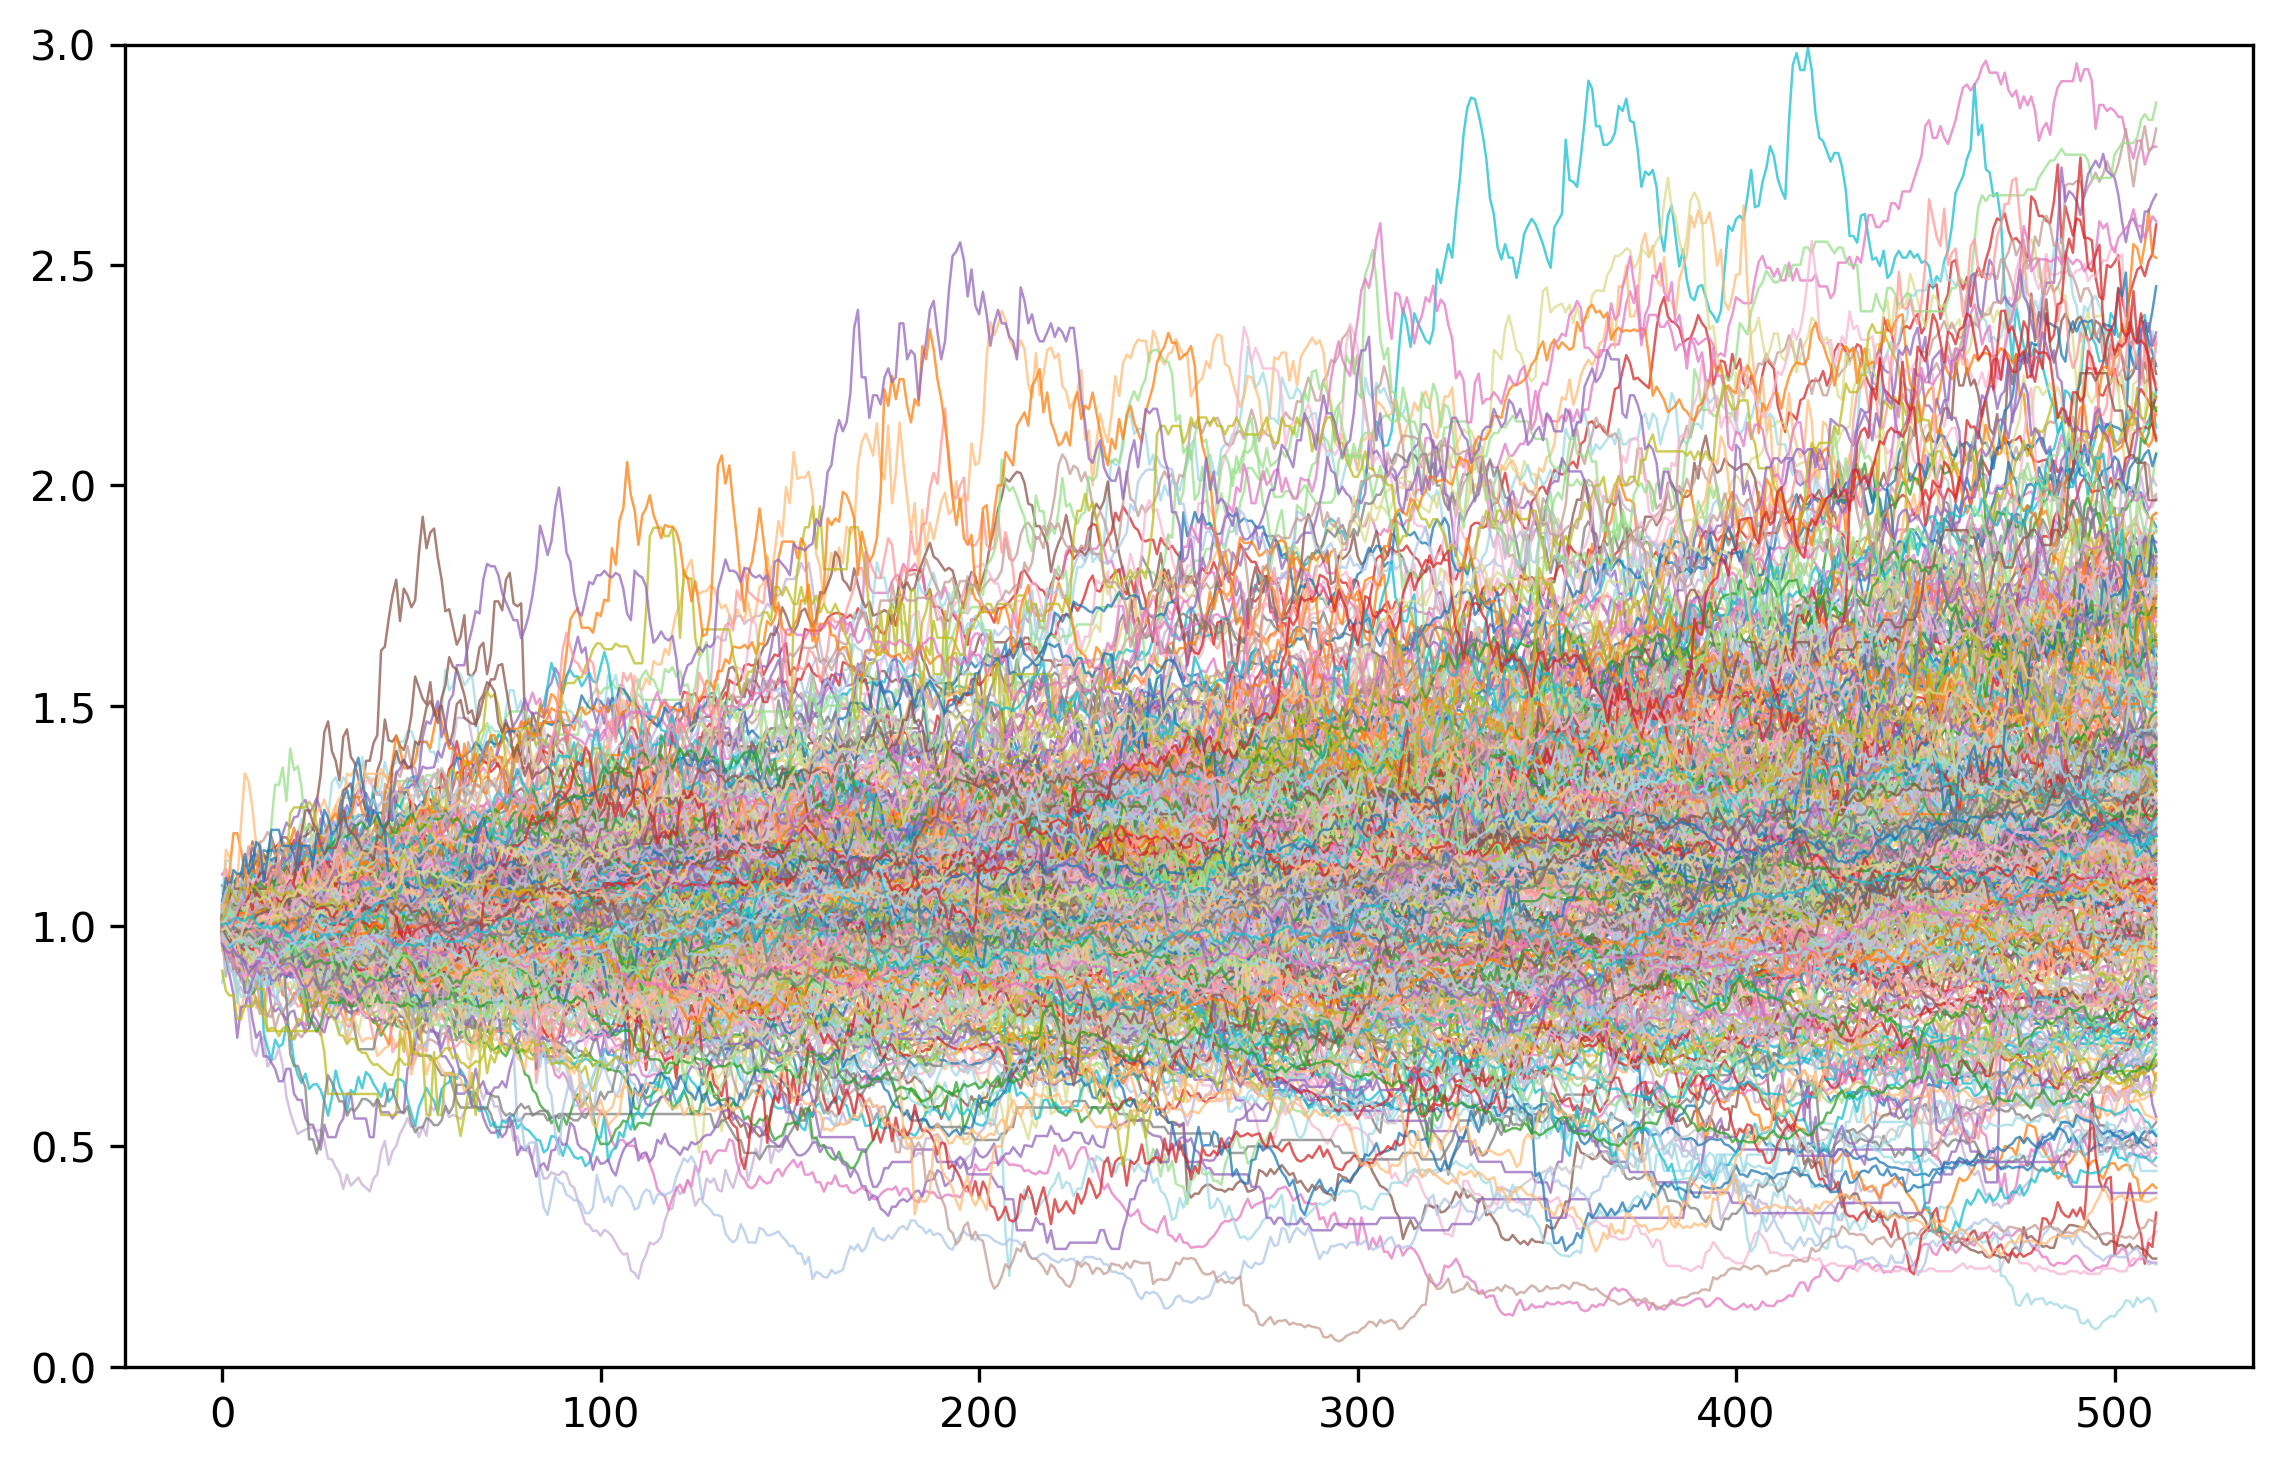
\includegraphics[width=\linewidth]{images/extra_experiments/price_paths_aggregate_reference.png}
        \caption*{Ground Truth}
        \label{fig:sampler_price_paths_gt}
    \end{subfigure}
    \hfill
    \begin{subfigure}[c]{0.32\textwidth}
        \centering
        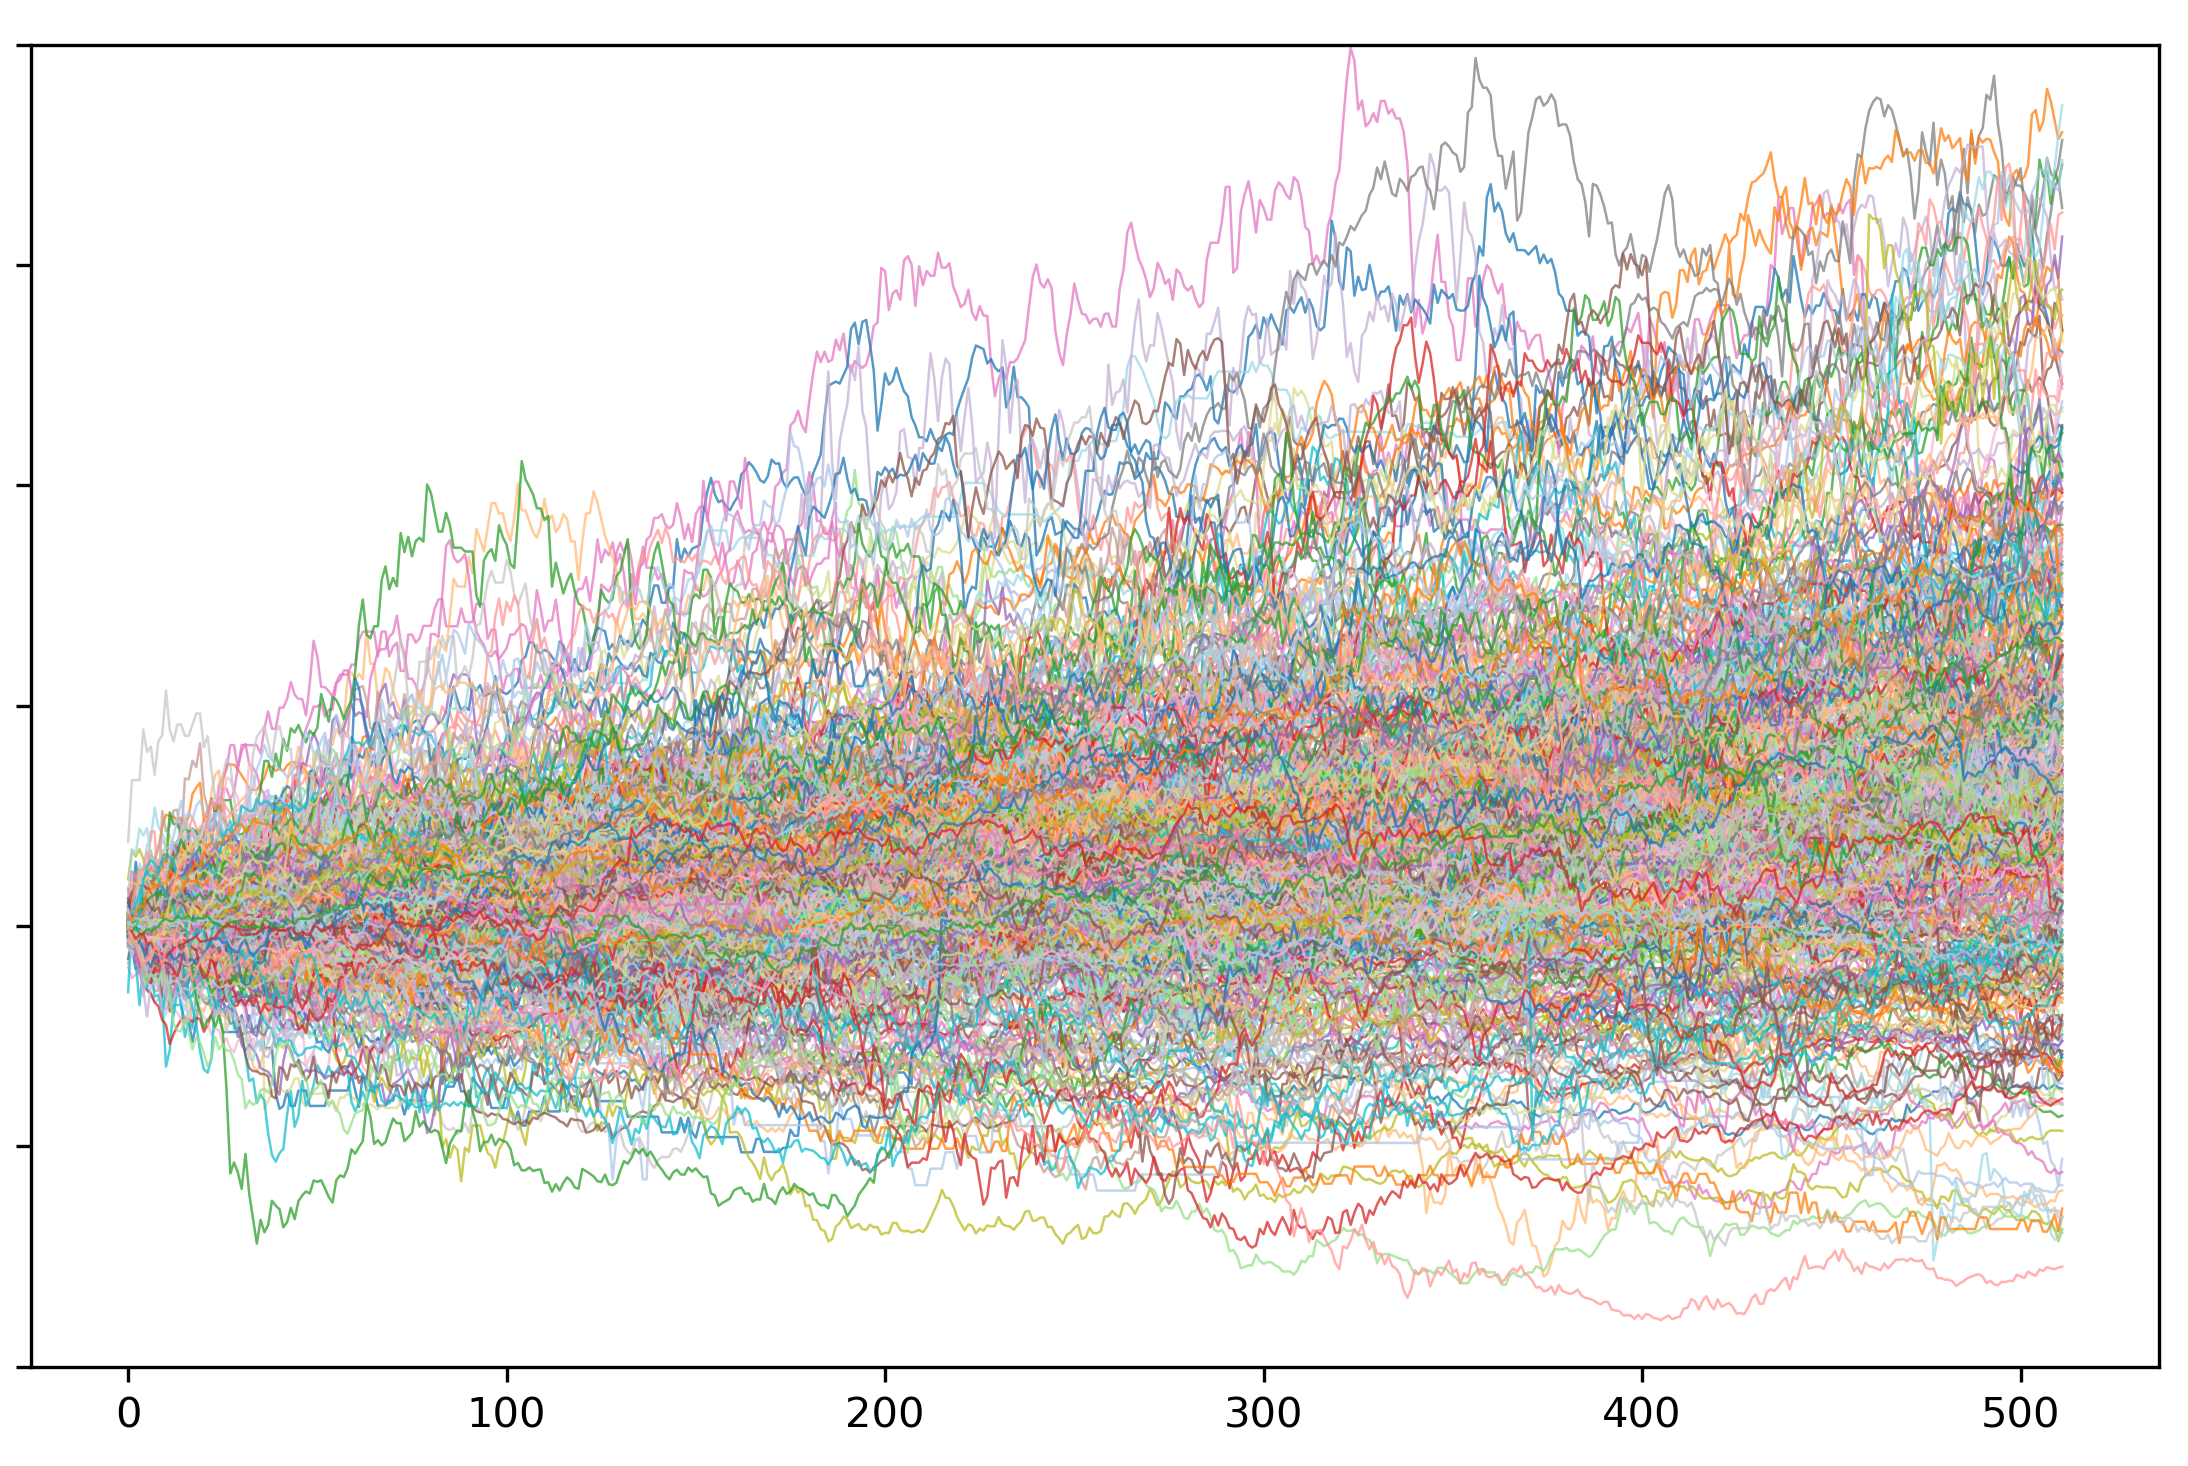
\includegraphics[width=\linewidth]{images/extra_experiments/price_paths_aggregate_reference_ODE.png}
        \caption*{Heun ODE}
        \label{fig:sampler_price_paths_ode}
    \end{subfigure}
    \hfill
    \begin{subfigure}[c]{0.32\textwidth}
        \centering
        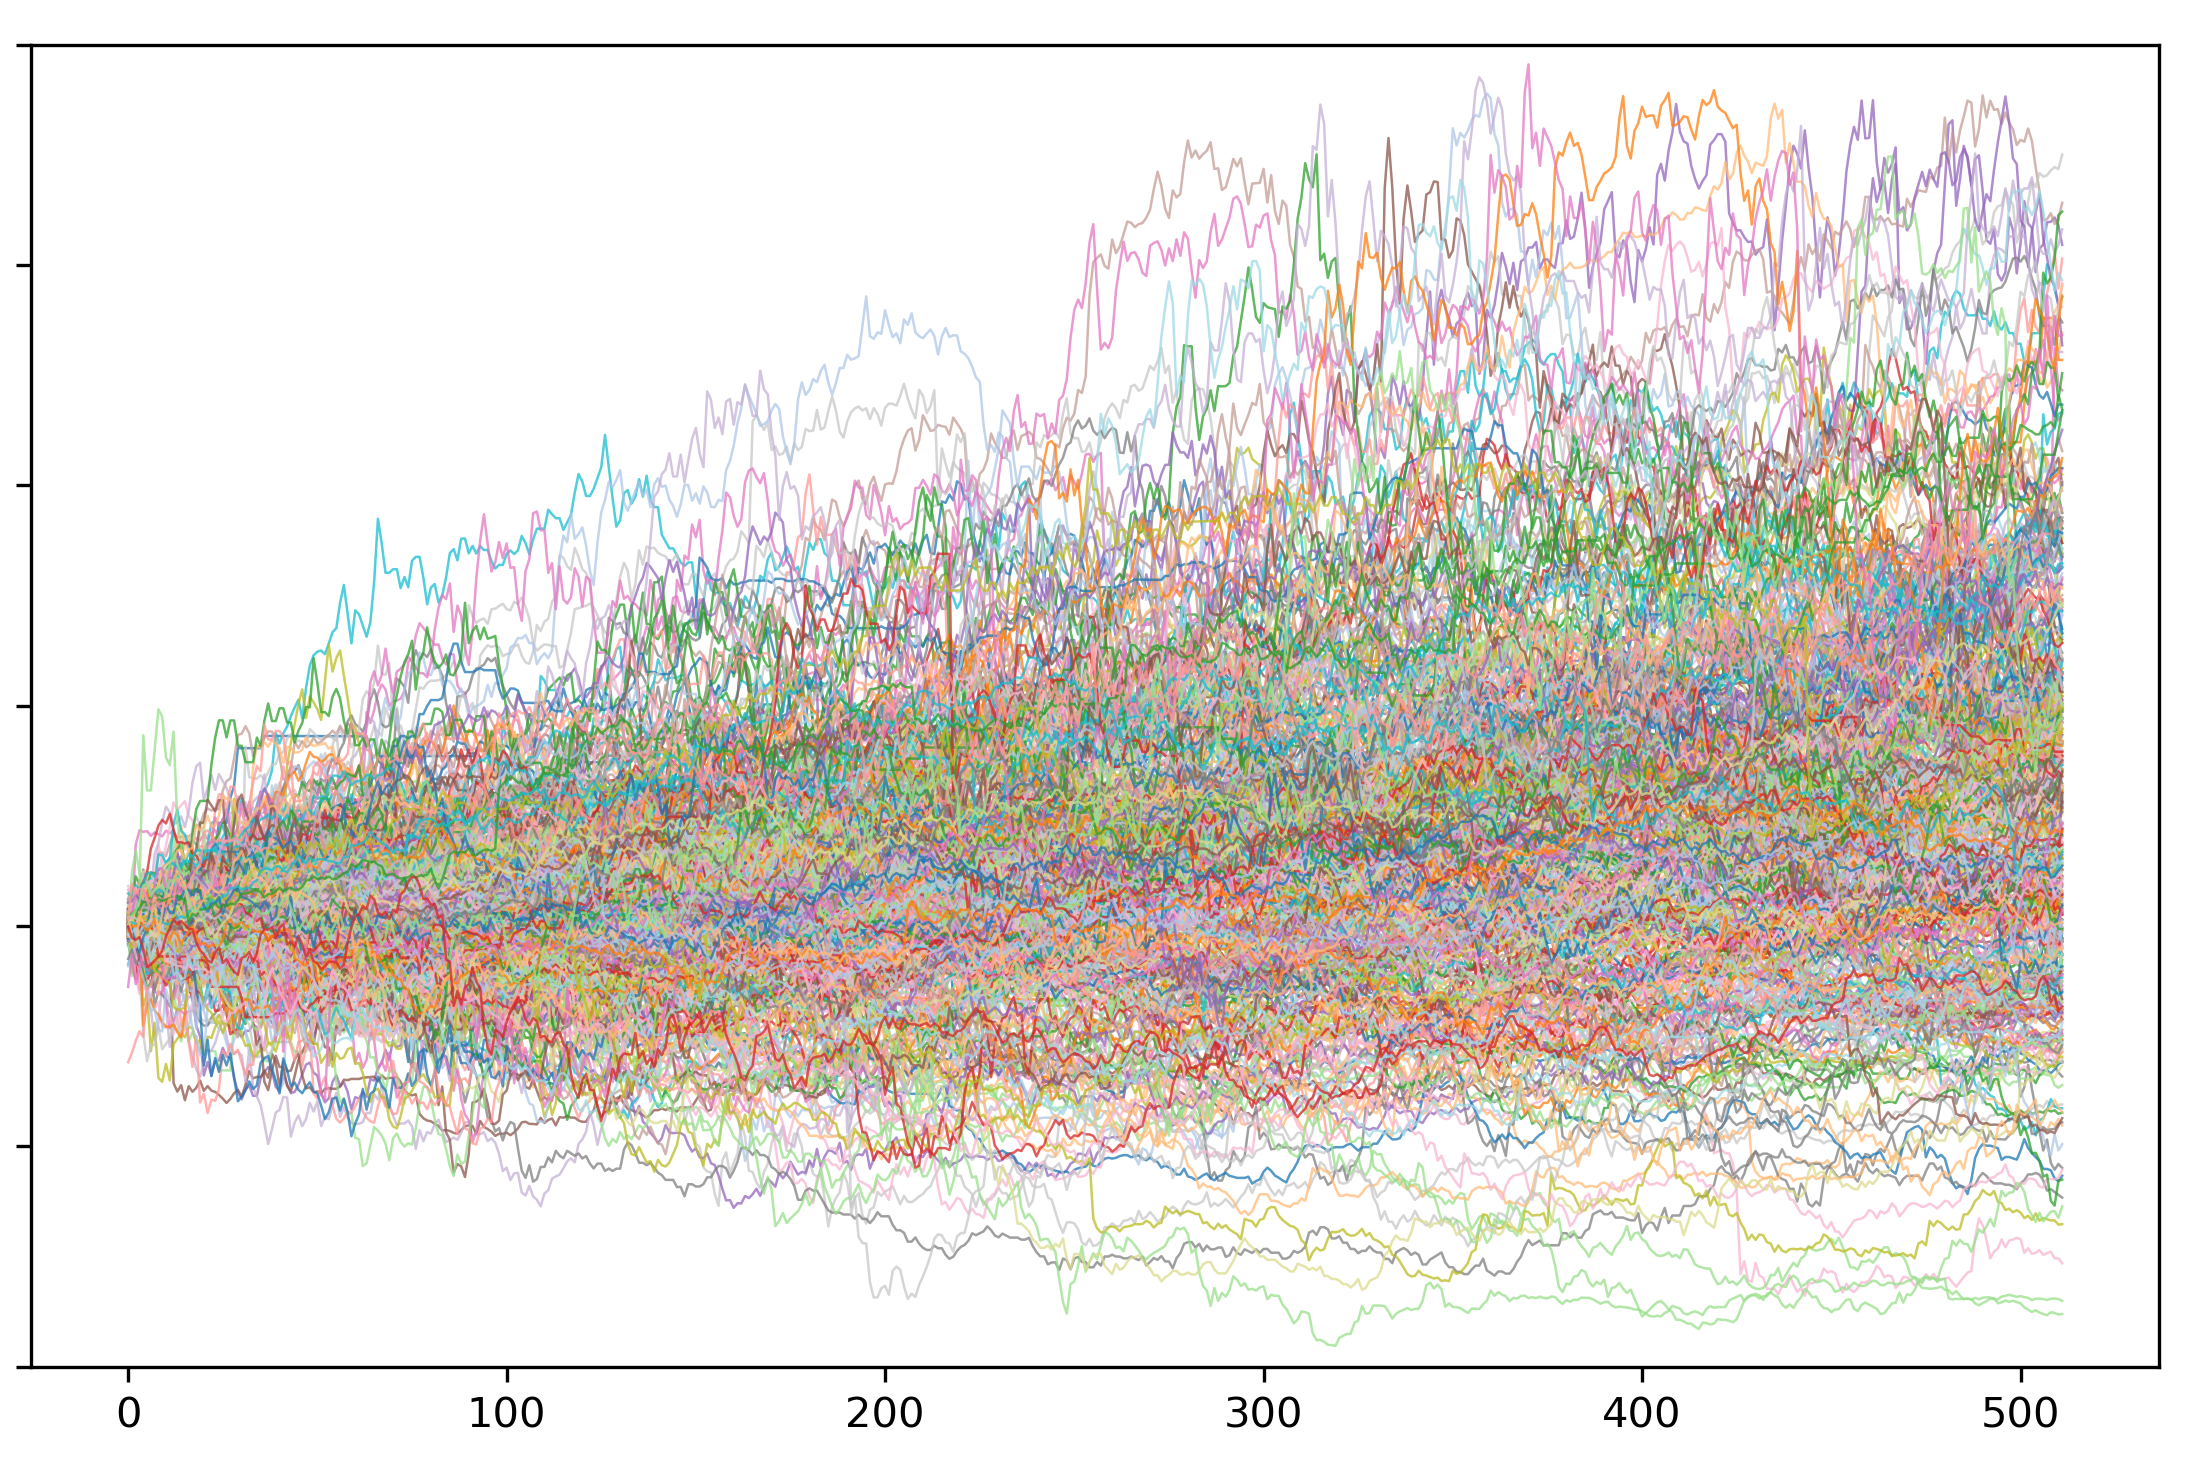
\includegraphics[width=\linewidth]{images/extra_experiments/price_paths_aggregate_reference_SDE.png}
        \caption*{Heun SDE}
        \label{fig:sampler_price_paths_sde}
    \end{subfigure}
    \caption{Sample price paths for EDM-CSDI (Cond.). \emph{Left}: Ground Truth. \emph{Centre}: Heun ODE. \emph{Right}: Heun SDE.}
    \label{fig:sampler_price_paths}
\end{figure}

\subsection{NFEs Variations}
Another set of experiments focused on sampling with EDM-CSDI (Cond.) under the Heun ODE sampler with a different number of function evaluations (NFEs), specifically \(NFEs=200\) (\(steps=100\)) and \(NFEs=600\) (\(steps=300\)), to evaluate whether any discernible difference would be observed with respect to the default configuration \(NFEs=400\) (\(steps=200\)) used in sub-Sec.\ \ref{subsec:conditiona_edm_csdi}. For computational-speed reasons given the HPC constraints, the generated set for this exploration was limited to \(10,000\) windows with \(5\) samples each (except for Heun ODE 400), rather than the full \(20,000\)-window set used elsewhere in this chapter.

\begin{table}[htbp]
\centering
\footnotesize
\renewcommand{\arraystretch}{1.3}
\setlength{\tabcolsep}{4.5pt}
\begin{tabular}{
  l
  S[table-format=3]      % NFEs
  S[table-format= 1.4]   % Mean:     ±0.xxxx
  S[table-format= 1.5]   % Std:      0.xxxxx
  S[table-format=-1.4]   % Skew.:   -x.xxxx
  S[table-format= 2.1]   % Kur.: xx.x
  S[table-format=-1.4]   % q01:     -x.xxxx
  S[table-format= 1.4]   % q99:      x.xxxx
}
\toprule
\textbf{Sampler}
  & \textbf{NFEs}
  & {\textbf{Mean}}
  & {\textbf{Std}}
  & {\textbf{Skew.}}
  & {\textbf{Kur.}}
  & {$\boldsymbol{q_{0.01}}$}
  & {$\boldsymbol{q_{0.99}}$} \\
\midrule
Reference & {---} &  0.0000 & 1.0000 & -0.5864 & 39.5 & -2.7188 & 2.7784 \\
Heun ODE & 200 &  0.0028 & 0.9490 & -0.5280 & 39.8 & -2.5800 & 2.6300 \\
Heun ODE & 400 &  0.0029 & 0.9487 & -0.5390 & 39.0 & -2.5789 & 2.6306 \\
Heun ODE & 600 &  0.0028 & 0.9490 & -0.5280 & 39.8 & -2.5800 & 2.6300 \\
\bottomrule
\end{tabular}
\caption{Aggregate statistics for EDM-CSDI (Cond.) under the Heun ODE sampler with varying numbers of function evaluations (NFEs), normalized log-returns, computed over all (training and validation) windows. \(NFEs=400\) (\(steps=200\)) is the default configuration used throughout this chapter and reproduces the Heun ODE row of Tab.~\ref{tab:sampler_experiment} (\(20,000\) windows, 5 samples each); \(NFEs=200\) (\(steps=100\)) and \(NFEs=600\) (\(steps=300\)) were generated on the reduced \(10,000\)-window, 5-samples-per-window set described above.}
\label{tab:nfe_experiment}
\end{table}

\begin{table}[htbp]
\centering
\footnotesize
\renewcommand{\arraystretch}{1.3}
\setlength{\tabcolsep}{4.5pt}
\begin{tabular}{
  % l
  l
  l                      % NFEs
  l                      % D_KS
  l                      % W1
  l                      % alpha
}
\toprule
    \textbf{Sampler}
  & \textbf{NFEs}
  & {$D_{\mathrm{KS}}$}
  & {$W_1$}
  & {$\hat{\alpha}$} \\
\midrule
Reference & {---} & {---} & {---} & 4.418 \\
Heun ODE & 200 & 0.0402 & 0.000558 & {---} \\
Heun ODE & 400 & 0.0411 & 0.000569 & 4.572 \\
Heun ODE & 600 & 0.0403 & 0.000561 & {---} \\
\bottomrule
\end{tabular}
\caption{Distributional similarity metrics ($D_{\mathrm{KS}}$, $W_1$, $\hat{\alpha}$) for EDM-CSDI (Cond.) under the Heun ODE sampler with varying NFEs (cf.\ Tab.~\ref{tab:nfe_experiment}). $D_{\mathrm{KS}}$ and $W_1$ are computed against the unnormalized training marginal. Cells marked {---} were not computed for this exploration.}
\label{tab:nfe_distributional_metrics}
\end{table}

As shown in Tab.\ \ref{tab:nfe_experiment}, all three NFE configurations are nearly indistinguishable from one another and from the Reference, with standard deviation, skewness, kurtosis, and tail quantiles all within a narrow band around the \(NFEs=400\) baseline.

Tab.\ \ref{tab:nfe_distributional_metrics} indicates that \(NFEs=200\) and \(NFEs=600\) yield marginally lower \(D_{\mathrm{KS}}\) and \(W_1\) than \(NFEs=400\). Overall, departing from \(NFEs=400\) in either direction does not yield a clear, consistent improvement; part of the observed differences may also be attributable to the reduced \(10,000\)-window evaluation set used for \(NFEs=200\) and \(NFEs=600\) rather than to the NFE budget itself. Nevertheless, decreasing the number of steps by 50\% does not seem to be causing lower generative performances.

% [TO BE COMPLETED] Section commented out until the sigma_max=10.0 results are available.
% \textbf{\(\sigma_{\max}\) Value} \quad Subsequently, different \(\sigma_{\max}\) values were experimented with, whose role has been explained in Sec.\ \ref{sec:training_config}.
%
% \begin{table}[htbp]
% \centering
% \footnotesize
% \renewcommand{\arraystretch}{1.3}
% \setlength{\tabcolsep}{4.5pt}
% \begin{tabular}{
%   l
%   S[table-format=2.1]    % sigma_max: x.x or xx.x
%   S[table-format= 1.4]   % Mean:     ±0.xxxx
%   S[table-format= 1.5]   % Std:      0.xxxxx
%   S[table-format=-1.4]   % Skew.:   -x.xxxx
%   S[table-format= 2.1]   % Kur.: xx.x
%   S[table-format=-1.4]   % q01:     -x.xxxx
%   S[table-format= 1.4]   % q99:      x.xxxx
% }
% \toprule
% \textbf{Sampler}
%   & \textbf{\(\sigma_{\max}\)}
%   & {\textbf{Mean}}
%   & {\textbf{Std}}
%   & {\textbf{Skew.}}
%   & {\textbf{Kur.}}
%   & {$\boldsymbol{q_{0.01}}$}
%   & {$\boldsymbol{q_{0.99}}$} \\
% \midrule
% Reference & {---} &  0.0000 & 1.0000 & -0.5864 & 39.5 & -2.7188 & 2.7784 \\
% Heun ODE & 8.0  &  0.0029 & 0.9487 & -0.5390 & 39.0 & -2.5789 & 2.6306 \\
% Heun ODE & 10.0 & & &  &  &  &  \\
% \bottomrule
% \end{tabular}
% \caption{Aggregate statistics for EDM-CSDI (Cond.) under varying $\sigma_{\max}$ priors with the second-order Heun ODE sampler, normalized log-returns, computed over all (training and validation) windows.
% $\sigma_{\max}=8.0$ corresponds to the default EDM configuration used
% throughout this chapter ($\sigma_{\max}=P_{\text{mean}}+5P_{\text{std}}$); results
% for $\sigma_{\max}=10.0$ are pending.}
% \label{tab:sigma_max_experiment}
% \end{table}
%%%%%%%%%%%%%%%%%%%%%%%%%%%%%%%%%%%%%%%%%%%%%%